\documentclass[a4paper,11pt]{article}
\usepackage{fullpage}
\usepackage{standalone}
\usepackage[utf8]{inputenc}
\usepackage[british]{babel}
\usepackage{csquotes}
\usepackage[T1]{fontenc}
\usepackage{amsmath}
\usepackage{amssymb}
\usepackage{mathtools}
\usepackage{mathptmx}
\usepackage{natbib}
\usepackage[final,babel]{microtype}
\usepackage[hidelinks]{hyperref}
\usepackage{doi}
\usepackage{siunitx}
\usepackage[margin=1pt]{subcaption}
\usepackage{xcolor}
\PassOptionsToPackage{final}{graphicx}
\usepackage{tikz}
\usetikzlibrary{arrows}
\usetikzlibrary{patterns}
\usepackage{bm}
\usepackage{booktabs}
\usepackage{tabularx}
\usepackage{enumitem}
\usepackage{kbordermatrix}
\usepackage{draftwatermark}

\title{
\vspace*{-2em}
Monitoring Committee Progress Report \#3\\
\vspace*{1em}
\Large{Numerical Representation of Mountains in Atmospheric Models}}
\author{James Shaw
\vspace{0.5em} \\
\large{Supervisors: Hilary Weller, John Methven, Terry Davies}
\vspace{0.5em} \\
\large{Monitoring Committee: Maarten Ambaum, Paul Williams}}
\date{31st May 2016}

\captionsetup{margin=3pt,font={small}}
\setlength{\bibsep}{0.25em plus 0.1ex}

\makeatletter
\AtBeginDocument{
  \hypersetup{
    pdftitle = {Monitoring Committee Progress Report \#3},
    pdfauthor = {James Shaw}
  }
}
\makeatother


\newcommand{\TODO}[1]{\textcolor{purple}{TODO: \emph{#1}}}
\begin{document}
\SetWatermarkLightness{0.95}
\newcommand{\exner}{\Pi}
\maketitle

\section{Introduction}

Next-generation atmospheric models are designed to be more flexible than previous models, so that the choice of mesh and choices of numerical schemes can be deferred or changed during operation \citep{ford2013,theurich2015}.
My PhD project seeks to make numerical weather and climate predictions more accurate by developing new meshes and numerical schemes that are suitable for next-generation models.
In particular, the project addresses the modelling of orographic flows on arbitrary meshes, focusing on three aspects: first, how orography is best represented by a mesh; second, how to accurately advect quantities over orography and, third, how to avoid unphysical solutions in the vertical balance between pressure and temperature.

\subsection*{Representing orography with meshes}

There are two main types of mesh used in atmospheric models: terrain-following meshes and cut cells meshes.
Terrain-following meshes reduce numerical accuracy in the calculation of horizontal pressure gradients \citep{gary1973,zaengl2012} and advection terms \citep{schaer2002}.  Inaccuracies are larger near steep terrain.
Cut cell meshes are an alternative to terrain-following meshes.  Cut cell meshes are orthogonal everywhere except at the surface so that pressure gradient errors and advection errors are reduced, especially near steep terrain \citep{lock2012,good2014}.  However, cut cell meshes can have arbitrarily small cells which impose severe constraints on the timestep for explicit methods or semi-implicit methods \citep{almgren1997}.

To illustrate the two types of mesh, a wave-shaped mountain with a peak height of \SI{1}{\kilo\meter} is represented using a basic terrain-following mesh (figure~\ref{fig:btf-mesh}) and a cut cell mesh (figure~\ref{fig:cutcell-mesh}).  Notice that the basic terrain-following mesh is severely distorted over steep surfaces while, on the cut cell mesh, small cells are found near the mountain peak.
The development of a new type of mesh, the slanted cell mesh, is discussed in section~\ref{sec:tf-slanted-cells}.

\subsection*{Advection on arbitrary meshes}
\TODO{rewrite this to focus on multidimensional schemes, and how ours is computationally cheaper than FFSL multidimensional schemes, such as CSLAM and lashley2002}
When a wind field is misaligned with the mesh, an advection scheme must account for transverse flux between diagonally adjacent cells \citep{clappier1998}.  Dimensionally split schemes that do not account for transverse fluxes can distort advected quantities \citep{leonard1993}.  These distortions are called `splitting errors'.  In contrast, multidimensional schemes naturally account for such fluxes by including cross terms in the flux calculations \citep{leonard1993}.

Dimensionally split schemes are attractive because they are often computationally efficient compared to multidimensional schemes \citep{bott2010}, and a number of improvements have been developed to alleviate splitting errors \citep{leonard1996,bott2010}.  The advection scheme by \citet{weller-shahrokhi2014} is a multidimensional scheme that achieves computational efficiency by precomputing fluxes using the mesh geometry only.  Some aspects of this scheme are being modified to improve stability and accuracy, and this is the subject of section~\ref{sec:advection}.

\subsection*{Vertical balance on arbitrary meshes}
Some numerical models are susceptible to computational modes which produce unphysical solutions.   Models that have a Lorenz vertical staggering of variables can suffer from one such computational mode \citep{arakawa-konor1996}.  The Charney--Phillips vertical staggering does not suffer from the Lorenz computational mode, but it has only been formulated on structured, quadrilateral meshes.  I intend to develop a generalisation of the Charney--Phillips staggering for arbitrary meshes, and the necessary tasks are outlined in section~\ref{sec:future}.

\begin{figure}
	\centering
	\subcaptionbox{Basic terrain-following mesh \label{fig:btf-mesh}}[.32\linewidth]{\includegraphics[width=2in]{../thermalAdvection-mesh-btf-1000m-250dz/constant/mesh.pdf}}
	\subcaptionbox{Cut cell mesh \label{fig:cutcell-mesh}}[.32\linewidth]{\includegraphics[width=2in]{../thermalAdvection-mesh-cutCell-1000m-250dz/constant/mesh.pdf}}
	\subcaptionbox{Slanted cell mesh \label{fig:slantedcell-mesh}}[.32\linewidth]{\includegraphics[width=2in]{../thermalAdvection-mesh-slantedCell-1000m-250dz/constant/mesh.pdf}}
	\caption{Cell edges of basic terrain-following, cut cell and slanted cell meshes having the same wave-shaped mountain profile.  Only the lowest \SI{1.2}{\kilo\meter} in the centre of the domain is shown.  The entire domain is \SI{300}{\kilo\meter} wide and \SI{30}{\kilo\meter} high.  Axis units are \si{\meter}.
The cut cell mesh was generated with code used in the All Scale Atmospheric Model \citep{jaehn2015}, kindly provided by the Leibniz Institute for Tropospheric Research.}
	\label{fig:meshes}
\end{figure}

\section{Comparison of terrain-following and slanted cell meshes}
\label{sec:tf-slanted-cells}

During the first year of my PhD, I compared the numerical accuracy on terrain-following and slanted cell meshes.
In the second monitoring committee report (called MC2 hereafter), a slanted cell mesh was referred to as a cut cell mesh, but it is necessary to make a distinction between the two types: the differences can be seen by comparing the representation of the same terrain profile using cut cells (figure~\ref{fig:cutcell-mesh}) and slanted cells (figure~\ref{fig:slantedcell-mesh}).

The slanted cell method has advantages over the cut cell method.
\citet{shaw-weller2016} was published in May 2016 and included the development of a new slanted cell mesh generation method which avoided the complex heuristics employed by the previous method (see MC2, section 3).
This method makes slanted cell meshes straightforward to construct, unlike the construction of cut cell meshes, which can be somewhat involved \citep{hartkopf2011}.  Second, slanted cell meshes alleviate the severe timestep constraints associated with cut cell meshes \citep{shaw-weller2016}.

\section{Improving advection on slanted cell meshes}
\label{sec:advection}

My current work focuses on improving the stability of a multidimensional advection scheme that is suitable for arbitrary meshes \citep{weller-shahrokhi2014}.  The performance of the advection scheme is being evaluated over steep slopes on terrain-following, cut cell and slanted cell meshes.

The multidimensional advection scheme is an explicit, Eulerian, finite-volume scheme that has a cubic upwind-biased stencil.  Fluxes across faces are approximated using a least squares polynomial fit onto the stencil point values.
On a two-dimensional quadrilateral mesh, the stencil has $4 \times 3$ points in the domain interior (figure~\ref{fig:stencil-interior}), but may include fewer points near the boundaries.  This is a particular concern at the lower boundary where stencils may be smaller and highly distorted (figure~\ref{fig:stencil-lower-boundary}).

\begin{figure}
	\centering
	\subcaptionbox{12-point stencil in the domain interior \label{fig:stencil-interior}}[.48\linewidth]{\documentclass[tikz]{standalone}
\usepackage{bm}
\begin{document}
\begin{tikzpicture}[
  scale=0.5,
  cpnt/.style={fill=gray},
]
\draw [thick, ->] (0,7.5) -- (2,7.5) node [midway, anchor=south] {$\mathbf{u}$};

\draw (0,0) -- (3,0) -- (3,2) -- (0,2) -- (0,0);
\draw (0,2) -- (3,2) -- (3,4) -- (0,4) -- (0,2);
\draw (0,4) -- (3,4) -- (3,6) -- (0,6) -- (0,4);

\draw (3,0) -- (6,1) -- (6,3) -- (3,2);
\draw (6,3) -- (6,5) -- (3,4);
\draw (6,5) -- (6,7) -- (3,6);

\draw (6,1) -- (9,3) -- (9,5) -- (6,3);
\draw (9,5) -- (9,7) -- (6,5);
\draw (9,7) -- (9,9) -- (6,7);

\draw (9,3) -- (12,4) -- (12,6) -- (9,5);
\draw (12,6) -- (12,8) -- (9,7);
\draw (12,8) -- (12,10) -- (9,9);

\draw [ultra thick] (9,5) -- (9,7);
\draw [thick] (9,6) circle [radius=0.15] node [anchor=west] {$F$};

\path [cpnt] (1.5,1) circle [radius=0.1];
\path [cpnt] (1.5,3) circle [radius=0.1];
\path [cpnt] (1.5,5) circle [radius=0.1];

\path [cpnt] (4.5,1.5) circle [radius=0.1];
\path [cpnt] (4.5,3.5) circle [radius=0.1];
\path [cpnt] (4.5,5.5) circle [radius=0.1];

\path [cpnt] (7.5,3) circle [radius=0.1];
\path [cpnt] (7.5,5) circle [radius=0.1];
\path [cpnt] (7.5,7) circle [radius=0.1];

\path [cpnt] (10.5,4.5) circle [radius=0.1];
\path [cpnt] (10.5,6.5) circle [radius=0.1];
\path [cpnt] (10.5,8.5) circle [radius=0.1];

\end{tikzpicture}
\end{document}
}
	\subcaptionbox{7-point stencil near the lower boundary of a slanted cell mesh.  The ground is shown with diagonal hatching. \label{fig:stencil-lower-boundary}}[.48\linewidth]{\vspace*{2em}\documentclass[tikz]{standalone}
\usepackage{bm}
\usetikzlibrary{patterns}
\begin{document}
\begin{tikzpicture}[
  scale=0.5,
  cpnt/.style={fill=gray},
]

\draw [thick, ->] (6,7) -- (8,7) node [midway, anchor=south] {$\mathbf{u}$};

\draw (9,0) -- (9,6) -- (3,6) -- (0,7) -- (3,3.8) -- (6,1) -- (9,0);
\draw (3,6) -- (3,3.8);
\draw (6,6) -- (6,1);
\draw (9,2) -- (6,2) -- (3,3.8);
\draw (9,4) -- (6,4) -- (3,3.8);

\fill [pattern=north east lines] (0,7) -- (3,3.8) -- (6,1) -- (9,0) -- (9,-0.5) -- (0,-0.5) -- (0,7);

\draw [ultra thick] (6,1) -- (6,2);
\draw [thick] (6,1.5) circle [radius=0.15] node [anchor=west] {$F$};

\path [cpnt] (2.2,5.5) circle [radius=0.1];

\path [cpnt] (5,2.3) circle [radius=0.1];
\path [cpnt] (5,3.3) circle [radius=0.1];
\path [cpnt] (4.4,4.9) circle [radius=0.1];

\path [cpnt] (7.5,1.3) circle [radius=0.1];
\path [cpnt] (7.5,3) circle [radius=0.1];
\path [cpnt] (7.5,5) circle [radius=0.1];

\end{tikzpicture}
\end{document}
}
	\caption{Two-dimensional stencils used for approximating a value at a face centroid given a set of surrounding cell centre values.  In the two stencils, the face $F$ is shown with a thick line, and the face centroid with an open circle. Cell centres are denoted by grey filled circles.  The direction of the windvector, $\bm{u}$, is shown above both stencils.}
	\label{fig:stencils}
\end{figure}

In the interior of a two-dimensional domain, we fit a polynomial surface to a stencil of a discrete scalar field $\phi$:
\begin{align}
	\phi = a_1 + a_2 x + a_3 y + a_4 x^2 + a_5 x y + a_6 y^2 + a_7 x^3 + a_8 x^2 y + a_9 x y^2 \label{eqn:polynomial}
\end{align}
where $\bm{a} = a_1 \ldots a_9$ are the unknown coefficients that are calculated from the least squares fit.  It may not be possible to fit all the polynomial terms to a stencil near the lower boundary because it includes fewer points.  With additional help from Philip Browne, I have developed a mathematical technique that removes certain high-order terms based on the stencil geometry.  We call this technique an `adaptive polynomial fit'.

The adaptive polynomial fit uses the stencil geometry to construct a full-rank matrix.  For a stencil in the interior of a two-dimensional domain with twelve points, $c_1 \ldots c_{12}$, the matrix $B$ is
\begin{align}
	B = 
	\kbordermatrix{
		& \mathrm{constant} & x & y & x^2 & x y & y^2 & x^3 & x^2 y & x y^2 \\
		c_1 & 1 & x_1 & y_1 & x_1^2 & \cdots & \cdots & \cdots & \cdots & x_1 y_1^2 \\
		c_2 & 1 & x_2 & y_2 & x_2^2 & \cdots & \cdots & \cdots & \cdots & x_2 y_2^2 \\
		\vdots & \vdots & \vdots & \vdots & \vdots &  &  &  &  & \vdots \\
		c_{12} & 1 & x_{12} & y_{12} & x_{12}^2 & \cdots & \cdots & \cdots & \cdots & x_{12} y_{12}^2 \\
	} \text{.}
\end{align}
Equation~\eqref{eqn:polynomial} is used to form a matrix equation $\bm{\phi} = B \bm{a}$, where $\bm{\phi}$ is the vector of stencil point values that can change between timesteps.
To solve for $\bm{a}$, the pseudo-inverse, $B^\dagger$, is calculated using the singular value decomposition of $B$.  Note that $B^\dagger$ can be precomputed using the stencil geometry alone.

For smaller stencils, or highly-distorted stencil geometries, the matrix $B$ may be numerically rank-deficient (that is, it has singular values close to zero).  To ensure that the matrix is full-rank, $B$ is constructed by appending one column at a time.  If any column causes the matrix to become rank-deficient then that column is omitted.  This technique constructs polynomial surfaces that are high-order for large, uniform stencils and lower-order for smaller stencils or highly-distorted stencils.

The adaptive polynomial fit alone is not enough to ensure numerical stability.  I am developing a new procedure that will stabilise the polynomial fit for troublesome stencils.  It is based on constraints derived from a one-dimensional von Neumann analysis of a simplified version of the spatial discretisation.  Compared to the original version of the advection scheme by \citet{weller-shahrokhi2014}, the improved version is stable for a wider range of test cases (figure~\ref{fig:instability}).  
However, the scheme is still weakly unstable in certain cases and work is ongoing to give us confidence that the scheme will be stable and accurate for arbitrary meshes.
I am also working with Tristan Pryer here at Reading, and I am reaching out to other experts in the field for suggested solutions.

\begin{figure}
\centering
\subcaptionbox{Improved scheme, $t = \SI{150}{\second}$ \label{fig:stable150}}[0.32\linewidth]{\hspace*{-1em}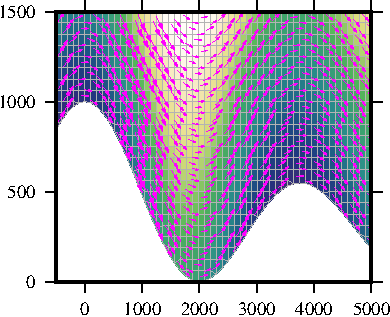
\includegraphics[width=2.25in]{slantedCellNew150.pdf}}
\subcaptionbox{Original scheme, $t = \SI{150}{\second}$ \label{fig:unstable150}}[0.32\linewidth]{\hspace*{1em}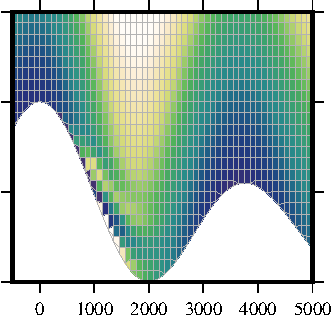
\includegraphics[width=1.9in]{slantedCellOld150.pdf}}
\subcaptionbox{Original scheme, $t = \SI{400}{\second}$ \label{fig:instability400}}[0.32\linewidth]{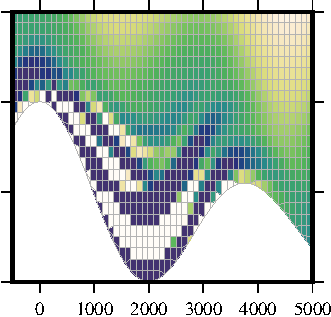
\includegraphics[width=1.9in]{slantedCell400.pdf}}
%
\vspace{1em} \\
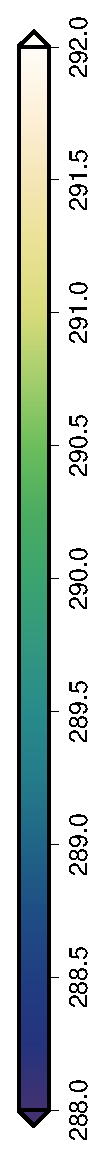
\includegraphics[height=5in,angle=270]{slantedCellLegend.eps}
%
	\caption{Comparison of results between the original advection scheme from \citet{weller-shahrokhi2014} and the improved advection scheme that includes the adaptive polynomial fit and stabilisation procedures.  After $t = \SI{150}{\second}$ the initial, stably-stratified thermal profile has been advected in a prescribed, terrain-following wind field over the wave-shaped mountains.  The new version of the scheme produces the expected result (\subref{fig:stable150}).  With the original version of the scheme, errors develop on the lee slope that are advected along the ground (\subref{fig:unstable150}).
By $t = \SI{400}{\second}$, the instability is fully-developed, having stripes of error and grid-scale oscillations that propagate in a direction opposite to the wind (\subref{fig:instability400}).
The timestep is \SI{2.5}{\second}.
Cell edges are shown by grey lines.  Wind vectors are drawn using magenta arrows, with the wind speed ranging from \SIrange{10}{13}{\meter\per\second}.  The wind field is the same for all results shown and the wind is time invariant.  Only the lowest \SI{1.5}{\kilo\meter} of the central domain is shown.  The entire domain is \SI{20}{\kilo\meter} wide and \SI{5}{\kilo\meter} high.  Axis units are \si{\meter}.}
\label{fig:instability}
\end{figure}

\section{Future research}
\label{sec:future}
A timeline of future work is presented with tentative completion dates for each group of tasks.
My future work begins with the completion of advection scheme development described in the previous section.  After that, I will resume my work developing advection schemes for generalised Charney--Phillips staggering on arbitrary meshes.
MC2 discussed some brief, exploratory work on this topic, but no further work has been done since then.

\begin{description}
\item[Autumn 2016]{Complete stabilisation of the multidimensional advection scheme.  We will submit a paper on the topic, noting that the advection scheme is computationally cheap and suitable for arbitrary meshes.  Advection tests will be performed over steep slopes and the advantages of the slanted cell mesh will be highlighted.}
%
\item[Spring 2017]{Develop a generalised Charney--Phillips staggering for arbitrary meshes.
This work comprises a series of tasks:
\begin{enumerate}
\item Define the prognostic variables and their arrangement on arbitrary meshes
\item Design a simple numerical scheme for advecting potential temperature
\item Incorporate the advection scheme into the fully-compressible model from \citet{weller-shahrokhi2014}, using a fully-explicit configuration
\item Compare the Lorenz and Charney--Phillips variants of the model by selecting test that excite the Lorenz computational model, such as the standing waves tests from \citet{arakawa-konor1996}
\end{enumerate}
Following this, further tasks should be undertaken if time permits:
\begin{enumerate}[resume]
\item Adapt the multidimensional cubic advection scheme for advecting potential temperature on generalised Charney--Phillips meshes
\item Modify the fully-compressible model to enable a semi-implicit configuration with the Charney--Phillips staggering
\end{enumerate}
}
\item[Summer 2017]{Write a thesis chapter documenting the generalised Charney--Phillips staggering, the advection scheme and associated work.}
\item[Winter 2017]{Prepare the thesis introduction and incorporate my other papers into the thesis.}
\item[Early 2018]{Complete PhD.}
\end{description}

\section{Personal development}
This section discusses some recent activities; a complete training record is provided in the appendix.
This year, I have attended almost all lunchtime and departmental seminars, HHH and mesoscale group meetings.  I take note of analytical techniques that might be useful in future, for example, verifying trends using low pass filters\footnote{The summer NAO in observations and CMIP models: impacts on European precipitation and uncertainties in future projected trends, Ileana Bladé, 7 March 2016}, and solving linear PDEs using Green's functions\footnote{Constraining ocean ventilation pathways and time scales with observations and models, Samar Khatiwala, 21 March 2016}.
I have also peer reviewed a Monthly Weather Review manuscript, and I am keen to get better at critically analysing papers.

Following a talk by Ed Hawkins and Tom Sizmur about online scientific communication, I have been sharing more of my thoughts on my blog and on Twitter\footnote{My blog is at \url{datumedge.co.uk} and my Twitter username is \href{https://twitter.com/hertzsprrrung}{@hertzsprrrung}}.  I have found Twitter to be especially useful for discovering contacts from a range of disciplines whose interests overlap with my research.


\bibliographystyle{ametsoc2014}                                                 
\bibliography{references}

\newpage

\section*{Appendix}

\subsection*{Mathematics modules}
\footnotesize
\begin{tabular}{l l l l}
Spring 2016	& MA3NAT & Numerical Analysis II & unassessed \\
Spring 2015	& MAMNSP & Numerical Solution of Partial Differential Equations  & 78\% \\
\end{tabular}

\subsection*{RRDP modules}
\begin{tabular}{l l}
24 Mar 2016	& Voice coaching: looking after your voice \\
26--27 Jan 2016 & Preparing to teach (introduction, marking \& feedback, leading small groups) \\
2 Dec 2015	& An essential guide to critical academic writing \\
17 Nov 2015	& Understanding the UK higher education context \\
19 May 2015	& How to avoid plagiarism \\
10 Mar 2015	& How to write a literature review \\
19 Feb 2015	& How to write a paper \\
\end{tabular}

\subsection*{External courses}
\begin{tabular}{l l}
June 2016 & Dynamical core intercomparison project summer school, NCAR \\
13 May 2016 & Peer review: the nuts and bolts, Sense about Science \\
June 2015 & Advanced numerical methods for Earth-system modelling, ECMWF \\
\end{tabular}

\subsection*{Conferences and workshops}
\begin{tabularx}{\linewidth}{l l X}
October 2016 & Speaker & Numerical and computational methods for simulation of all-scale geophysical flows, ECMWF \\
July 2016 & Attendee & 1st GungHo Network meeting, Daresbury Laboratory \\
November 2015 & Attendee & GungHo workshop on next generation weather and climate prediction, UK Met Office \\
June 2015 & Attendee & Hoskins@70 \\
June 2015 & Poster & SCENARIO DTP conference \\
March 2015 & Speaker & Galerkin methods with applications in weather and climate forecasting, ICMS \\
\end{tabularx}

\subsection*{Teaching}
\begin{tabular}{l l l}
Oct 2015 & Teaching assistant & MTMG02 atmospheric physics \\
Sep 2015 & Teaching assistant & NCAS summer school \\
Sep 2014 & Course teacher & MPE python and linux short course \\
\end{tabular}

\subsection*{Visits and collaborations}
\begin{tabularx}{\linewidth}{l X}
July 2016 & Organising visit from Simon Clark, stratospheric PhD researcher and YouTube vlogger \\
June 2016 --\ & Working with Hilary's new MSc student, Christiana Skea, studying variable timestepping for ODEs \\
June 2016 & Visiting NCAR, hosted by Ram Nair \\
2015 -- 2016 & Coauthoring an article about dimensionally-split and multidimensional advection schemes, written with Hilary, her former student Yumeng Chen, and Stephen Pring at the UK Met Office \\
\end{tabularx}


\subsection*{Outreach}
\begin{tabular}{l l l}
14 Jul 2015 & Schools physicist of the year awards \\
14 Jun 2015 & East Reading festival \\
15 Feb 2015 & Brighton science festival \\
\end{tabular}

\subsection*{Presentations}
\begin{tabularx}{\linewidth}{l l X}
23 Mar 2016 & Quo Vadis & Numerical representation of orography in dynamical cores (honourable mention) \\
17 Feb 2016 & PhD group & Multidimensional advection schemes for arbitrary meshes \\
9 Feb 2016 & Mesoscale group & Curl-free pressure gradients for accurate modelling of cold air pools \\
19 Oct 2015 & HHH group & Improving modelled mountain flows with alternative representations of terrain \\
27 Apr 2015 & HHH group & A like-for-like comparison between terrain following and cut cell grids \\
21 Apr 2015 & PhD group & Discrete vector calculus on Arakawa C grids \\
12 Feb 2015 & UK Met office & Poster presentation \\
18 Jan 2015 & PhD group & Python and linux tips \\
17 Dec 2014 & MPECDT jamboree & Poster presentation \\
12 Sep 2014 & Lunchtime seminar  & Gain control of your documents and code: hands-on with revision control and build automation \\
\end{tabularx}

\end{document}
